\documentclass[12pt]{article}
\usepackage{amsmath}
\usepackage{euler}
\usepackage{authblk}
\usepackage{tikz}
\usetikzlibrary{positioning}

\usepackage{hyperref}
\hypersetup{
    colorlinks,
    citecolor=black,
    filecolor=black,
    linkcolor=black,
    urlcolor=black
}

\usepackage{bookmark}
\usepackage{cite}
\usepackage{fancyhdr}

\usepackage[margin=1.13in]{geometry}

\pagestyle{fancy}
\fancyhf{}
\rhead{\rightmark}

\usepackage{titlesec}
\titleformat{\chapter}[display]
  {\normalfont\bfseries}{}{0pt}{\Huge}
\author{Junlong Gao}
\affil{}
\date{}

\newcommand{\Lconsistent}{linearizability }
\newcommand{\Sconsistent}{serializability }
\newcommand{\LConsistent}{Linearizability }
\newcommand{\SConsistent}{Serializability }

\newcommand{\wip}[1]{\textcolor{red}{[\textit{TODO: #1}]}}

\begin{document}
\tableofcontents

\title{Considerations of Building Services on a Consensus Protocol}
\maketitle

Data redundancy is one of the most important techniques for achieving
fault-tolerance. Yet, redundancy complicates the access path for data as
replication posses challenges to maintain an illusion of ``single-copy''.
Under the standard fail-stop model, there is a limit where we cannot achieve
all three of \Lconsistent, availability, and partition tolerance. Despite the
impossibility, a class of quorum-based consensus protocols are widely adopted
in practice to implement a replicated log~\cite{lampson1996build}, which in
term allow us to build replicated state machines as a form of redundancy.
This small article explores some consensus protocols as well as how data
services are built on top of these replicated logs.

\section{Replicated Logs and Replicated State Machines}
\wip{Give an overview of how replicated logs can be used to build redundancy,
and hot raft works}

\section{Considerations of Building Services on a Consensus Protocol}
The replicated state machine is not the silver bullet of building fault
tolerant systems. Usually more complicated services are built on top of the
Raft stack.
Common architecture uses Raft to replicate a storage engine like LSM tree,
and build a state-less server on top of it to serve a richer storage
semantics.
For example, the client can implement a file system using the Raft nodes, and
the replicated state machine is the file system tree. The client itself
further exposes a service for the file system access protocol.

When reasoning concurrent objects, \Lconsistent is one of the most widely
used and suitable to programmer's intuition for consistency semantics. There
is a rich collection of literature of formalizing its
guarantees~\cite{herlihy1990linearizability, herlihy2011art}. In layman's
term and the purpose of this article, a state machine access is considered
\Lconsistent if for any collection of concurrent operations' histories
(request-response pairs) satisfies:
\begin{itemize}
    \item The effects of each operation in the histories seems to take effect
    at some point in that request-response pair (linearaization point);
    \item If $e_1^{reply}$ happens after $e_2^{request}$, then their
    linearaiation point have the same relative ordering (real-time).
\end{itemize}

There are 2 challenges in this architecture for implementing linearizability.
The first issue is the state machine linearizability problem: when the server
access the underlying replicated state like using raft protocol, how and
where should the read request be executed? Further, can this server cache the
read results without going to the replication layer? As we shall see in
Section \ref{sml} they are closely related and can be saved together.

The second problem lies in the exactly-once semantics: when concurrent
clients access the state machine, idempotent operations with retry is
insufficient to guarantee linearizability. An idempotent operation is not the
same as an exactly-once operation. For example, a POSIX \texttt{pwrite} is
the same if executed with the same parameters for multiple times and
considered as idempotent. However, it is not exactly-once as data is truly
written multiple times when \texttt{pwrite} is executed multiple times. On
the other hand, if there is a sequence number associated with the
\texttt{pwrite} command, it can be made exactly-once if a command with
eariler sequence number is ignored.

Retrying idempotent but not exactly-once operations over a central server can
result in at least 2 anomalies in terms of linearizability: one is
``resurrected write'', and another being ``out-of-order writes''. Figure
\ref{fig:M1} gives an example of resurrected write: the history is not
linearaizable as the write from $P_1$ is retried and ``resurrected'' and
observed. There is no way to find a linearaization point for $W(1)$ in its
request response pair as it has to be before the first observable state
$R(1)$, then after $W(2)$ the history contracts the second $R(1)$ in $P_2$.

The second anomaly ``out-of-order writes'' happens when 2 clients retries
their writes in the different order as they are observed when they are first
serialized in the server. \wip{ add a graph here}


\begin{figure}
    \centering
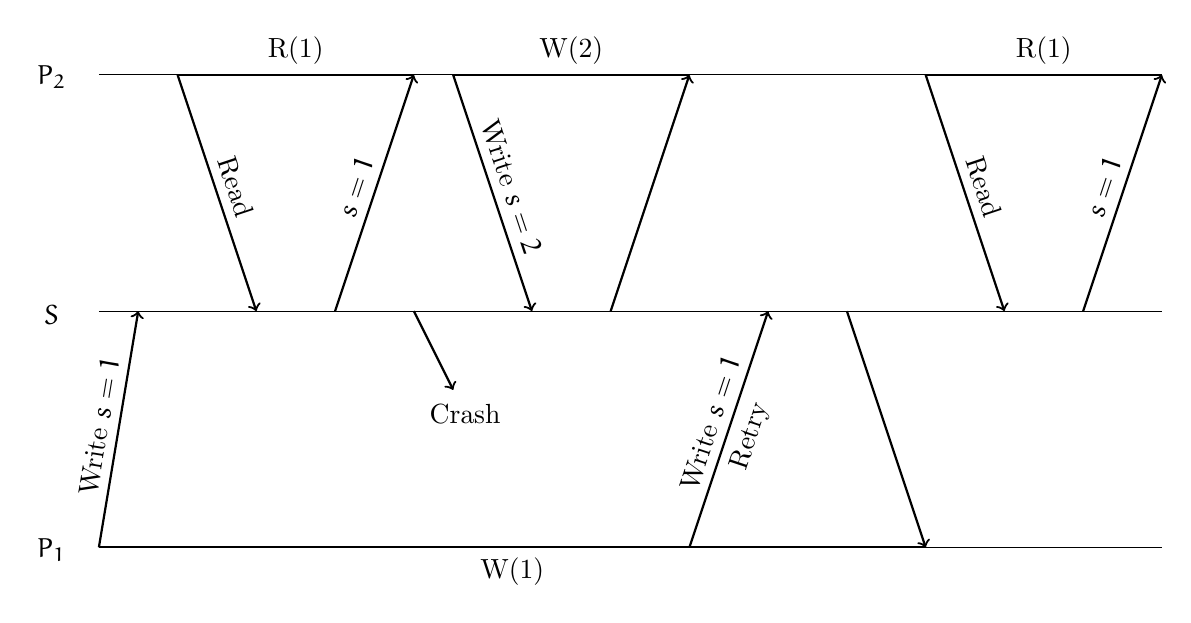
\begin{tikzpicture}
    \coordinate [label={[xshift=-0.6cm, yshift=-0.3cm]$P_1$}] (P1Begin) at (0,0);
    \coordinate (P1End) at (13.5,0);

    \coordinate [label={[xshift=-0.6cm, yshift=-0.3cm]$P_2$}] (P2Begin) at (0,6);
    \coordinate (P2End) at (13.5,6);

    \coordinate [label={[xshift=-0.6cm, yshift=-0.3cm]$S$}] (SBegin) at (0,3);
    \coordinate (SEnd) at (13.5,3);

    \coordinate (initVal) at (0, 3);

    \coordinate (P1_W1) at (0,0);
    \coordinate (S_Get_P1_W1) at (0.5, 3);

    \coordinate (P2_R1) at (1,6);
    \coordinate (S_Get_P2_R1) at (2,3);
    \coordinate (S_Reply_P2_R1) at (3,3);
    \coordinate (P2_Get_R1_Reply) at (4,6);

    \coordinate (SCrash) at (4,3);
    \coordinate (SCrash_End) at (4.5,2);

    \coordinate (P2_W2) at (4.5,6);
    \coordinate (S_Get_P2_W2) at (5.5,3);
    \coordinate (S_Reply_P2_W2) at (6.5,3);
    \coordinate (P2_Get_W2_Reply) at (7.5,6);

    \coordinate (P1_W1_Retry) at (7.5,0);
    \coordinate (S_Get_P1_W1_Retry) at (8.5, 3);
    \coordinate (S_Reply_P1_W1_Retry) at (9.5, 3);
    \coordinate (P1_Get_W1_Retry_Reply) at (10.5, 0);

    \coordinate (P2_R1_2) at (10.5,6);
    \coordinate (S_Get_P2_R1_2) at (11.5,3);
    \coordinate (S_Reply_P2_R1_2) at (12.5,3);
    \coordinate (P2_Get_R1_Reply_2) at (13.5,6);

    %Lines
    \draw[-] (P1Begin) -- (P1End);
    \draw[-] (P2Begin) -- (P2End);
    \draw[-] (SBegin) -- (SEnd);

    \draw[->, thick] (P1_W1) -- (S_Get_P1_W1)
       node[midway, above, sloped]
       {Write $s = 1$};

    \draw[->, thick] (P2_R1) -- (S_Get_P2_R1)
       node[midway, above, sloped]
       {Read};
    \draw[->, thick] (S_Reply_P2_R1) -- (P2_Get_R1_Reply)
       node[midway, above, sloped]
       {$s = 1$};

    \draw[->, thick] (P2_W2) -- (S_Get_P2_W2)
       node[midway, above, sloped]
       {Write $s = 2$};
    \draw[->, thick] (S_Reply_P2_W2) -- (P2_Get_W2_Reply)
        ;

    \draw[->, thick] (P1_W1_Retry) -- (S_Get_P1_W1_Retry)
       node[midway, above, sloped]
       {Write $s = 1$}
       node[midway, below, sloped]
       {Retry};
    \draw[->, thick] (S_Reply_P1_W1_Retry) -- (P1_Get_W1_Retry_Reply);

    \draw[->, thick] (P2_R1_2) -- (S_Get_P2_R1_2)
       node[midway, above, sloped]
       {Read};
    \draw[->, thick] (S_Reply_P2_R1_2) -- (P2_Get_R1_Reply_2)
       node[midway, above, sloped]
       {$s = 1$};

    \draw[->, thick] (SCrash) -- (SCrash_End)
       node[pos=1.3]
       {Crash};

    \draw[-, thick] (P1_W1) -- (P1_Get_W1_Retry_Reply)
       node[midway, below, sloped]
       {W(1)};

    \draw[-, thick] (P2_R1) -- (P2_Get_R1_Reply)
       node[midway, above, sloped]
       {R(1)};

    \draw[-, thick] (P2_W2) -- (P2_Get_W2_Reply)
       node[midway, above, sloped]
       {W(2)};

    \draw[-, thick] (P2_R1_2) -- (P2_Get_R1_Reply_2)
       node[midway, above, sloped]
       {R(1)};
\end{tikzpicture}
\caption{Example of Violating Linearizability with Idempotent Requests}
\label{fig:M1}
\end{figure}


\section{State Machine \LConsistent}\label{sml}
How should read and write be executed on the replicated log?
With replication which of the replica can execute mutation and propagate to
all the remaining nodes? Which of the replica can serve read of the state
machine? To provide high availability, the client may pick a different
replica for accessing the state machine.

Second, if the server is a file system daemon built on top of this
replicated log, can this file system daemon cache for reads? The file system
daemon can simply follow the leader, so it seems to be obvious that the
daemon serve reads directly for cached data, save a trip to the Raft node. A
closer look reveals this is not the case. When the leader switches, there
will be a small window that the client does not know (outside polling window)
and can serve a read from the local cache. In this case, the data could have
been overwritten by the new leader. This will violate linearizability \wip{
add a graph here}.

For the first question, leader based consensus protocols like Raft solve this
problem by only allowing the leader to take access requests. Then leader acts
as the linearaization point for all the operations: leader takes each
request, generate a log, and replicate it into the replicated log and apply
it to the state machine. However, it is now requiring read operations also
ending up in the replicated log. In this way read operations can be
serialized and ordered with the write operations in the log, and the complete
access path is now linearaizable.

Can we execute read on any non-leader node? Directly looking at the state
machine of a follower node is dangerous as the follower may not have received
the last write request from the leader. This is because write only need
majority to declare committed (well, there is more to that). Can we execute
read on leader node directly? Even after we received the ack from the leader
node, we may still risk failing with non-\Lconsistent behavior. If the read
is taking long enough, the leader can be part of the minority with the
client, unaware of what has been changed in the new leader. Putting read into
the replication protocols will detect this, but it is too expensive, because
this involves not only synchronously waiting for the majority, but also
incurs disk writes.

The \textit{ReadIndex} approach detailed in the original
thesis~\cite{ongaro2014consensus} partly solves this problem by avoiding the
log write. When the leader receives the read request, for it to be \Lconsistent,
there are 2 things to be established:
\begin{itemize}
    \item There cannot exist a newer committed state than the leader's commit
    index. \LConsistent requires read to reflect the state machine's state
    latest committed state (writes whose respond event is before the request
    event of the read), otherwise there is no way to pick a linearaization
    point for the read request that latest write request.
    \item The state machine must have a state not older than the leader
    commit index.
\end{itemize}
let the leader's commit index when it receives the read request be the
\textit{ReadIndex}, to establish the above two for that ReadIndex, it needs to
send a round of heartbeat and receive the majority confirming it is the
leader of the current term. Then wait for the state machine to apply through
the ReadIndex. After these two operations, the leader can respond by reading
off from the state machine.

After the above two is established, the leader can serve the read even if the
leader node suddenly loses the leader role. This is because any write must
happen after the new leader getting elected, and the new leader must appear after
the majority response the heartbeat. Therefore, the request event of the new
write is \textit{after} the request event of the read request. Then the read
request can be linearized by taking the linearaization point as the beginning
of the read request.

From the idea of ReadIndex, we can take it further for two extensions. The first
one is follower-read. Replicas can serve read to reduce leader workload. This can
be done by allowing the follower to request a readIndex from the leader. Leader in
this case just need to issue a majority heartbeat and respond the ReadIndex after
success. Then the follower can wait until its state machine to be advanced to the
ReadIndex and serve the read. These can be heavily batched to improve throughput.

The second one is to avoid the majority heartbeat altogether from the leader
read. This requires additional assumptions though. One can assume bounded
clock drift (measured by the absolute error per second). Clock drift is the
difference in clock speed between nodes. At time $t_1$, node $A$ is the
leader. If we assume clock drift is $T_{drift}$ and leader timeout is
$T_{timeout}$, then we know the next write cannot happen until $t_1 +
\textrm{max}(T_{timeout}, T_{timeout} / T_{drift})$. Call this
$t_{lower}(t_1)$ as it is the lower-bound of the next write's timestamp. If
we ignore relativistic effects, the leader can always advance $t_{lower}(t)$
on a regular heartbeat basis. As long as the state machine is caught up with
the commit index, the read can be served without the additional round trip to
the majority. Of course, in reality due to hardware differences and GC
pauses, the bound is not so easy to maintain. Unless, a robust and powerful time
service is built for this purpose~\cite{Cooper_2013}.

Clients can also issue ``Snapshot Read'' if it uses the commit index
return from the leader for each write. Then the client can talk to any node
to issue a read with that index. This will at least allow the client observe
its own latest update (if a node does not have that index applied in the
state machine, just ask the client to retry a different node) and maintain
sequential consistency.


\section{Re-sync}
\wip{explain how raft resync state in the committed log when a node is catching up}

\bibliography{main}{}
\bibliographystyle{plain}
\end{document}
